
\chapter{Aparelho Fonador}
\section{Anatomia da Voz}
	Para estudar a produção e a síntese da voz, é necessário ter um conhecimento acerca da anatomia e do funcionamento físico da voz \citenum{Foundation1}. Sendo assim, as subseções seguintes descreverão brevemente detalhes da anatomia do sistema fonador humano e como o som é produzido, moldado e influenciado por este sistema.
	
	\begin{figure}
		\centering
		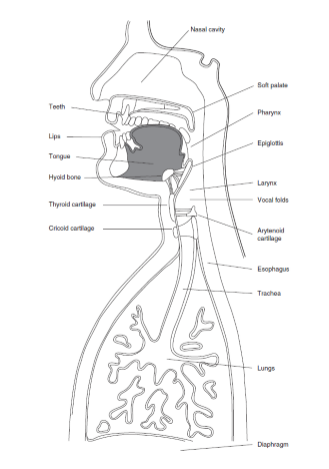
\includegraphics[scale=0.5]{aparelhoFonador}
		\caption{Aparelho Fonador}
		\label{fig:aparelhoFonador}
	\end{figure}
	\subsection{Aparelho Fonador}
	O estudo do aparelho fonador começa-se por suas estruturas e componentes importantes. Após um estudo detalhado dos fenômenos físicos e como se comportam é essencial também.
		
	A Figura \ref{fig:aparelhoFonador} \citenum{Foundation1}, mostra os órgãos associados com a produção da voz. 
	
	Dentro das condições normais, a voz é produzida quando um fluxo de ar vindo dos pulmões é convertido em energia acústica através da vibração das pregas vocais, localizadas na laringe. Os padrões de vibrações resultantes são moldados acusticamente quando o som passa pelo trato vocal acima da laringe. O sistema respiratório serve como uma
	fonte de potência para a produção do som, sendo responsável por movimentar o ar através do trato vocal. A laringe atua como um oscilador convertendo a potência aerodinâmica produzida em energia sonora, sendo frequentemente retratada como a fonte da voz. No entanto, a mais importante função da laringe não é a produção de som, e sim, vedar as vias aéreas aos pulmões completamente, protegendo-as de objetos estranhos ou líquidos, principalmente durante a deglutinação. De maneira análoga, a laringe serve como uma válvula de acesso às vias respiratórias e por essa característica, atua também no controle do fluxo de ar que por elas passam. Sendo assim,é fácil notar que há uma necessidade de mobilidade para toda estruturada laringe, logo é de se esperar que sua estrutura seja formada em sua maioria por cartilagens. De fato o é, com exceção de um osso chamado de Hioide, a laringe é basicamente formada por cartilagens e músculos. A seguir, analisaremos brevemente a dinâmica dos músculos e cartilagens da laringe.
	
\subsection{Músculos e Cartilagens}
Os músculos e cartilagens atuam diretamente no processo de abdução e adução das pregas vocais. Estas estão localizadas dentro da laringe e devido à dinâmica das cartilagens e dos músculos, podem executar os movimentos citados de forma a produzir som.

\subsubsection{Cartilagens da Laringe }
\begin{figure}
	\centering
	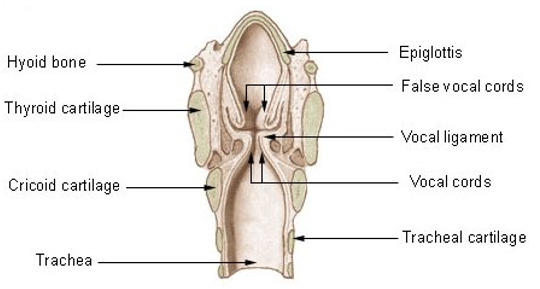
\includegraphics[scale=0.5]{musculosCartilagens}
	\caption{Secção coronal da laringe e parte superior da traquéia}
	\label{fig:Cartilagens}
\end{figure}
A Figura \ref{fig:Cartilagens}, mostra uma secção da laringe, detalhando as cartilagens presentes.
De maneira sucinta, estas cartilagens servem como base de interconexão para os músculos intrínsecos ao redor da laringe. Dentre as cartilagens acima, a epiglote é responsável por vedar as vias respiratórias movimentando-se sobre a entrada das mesmas. O resto das cartilagens garantem a mobilidade da laringe em conjunto com outras estruturas como por exemplo o sternum.


\subsubsection{Músculos da Laringe}
Os músculos na laringe podem ser divididos em dois grupos, os intrínsecos e os extrínsecos \citealp{Giovanni20041}. Os músculos intrínsecos interconectam as cartilagens da laringe, ao passo que, os extrínsecos conectam a laringe à outras estruturas externas, como o osso hióide. A Figura \ref*{fig:musculos} detalha alguns dos músculos intrínsecos da laringe. Alguns desses músculos têm influência direta em algumas características da voz. Por exemplo, o músculo cricotiroideo é o músculo primário utilizado no controle do tom da voz. Por sua vez, o músculo cricoaritenoideo posterior atua na abdução das pregas vocais, ao passo que o músculo interaritenoideo atua como adutor das pregas vocais.

\begin{figure}
	\centering
	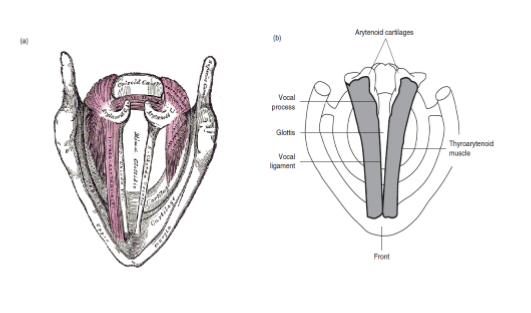
\includegraphics[scale=0.5]{musculosLaringe}
	\caption{Músculos Intrínsecos da Laringe}
	\label{fig:musculos}
\end{figure}

Os músculos extrínsecos, Figura \ref{fig:musculoExterno}, atuam basicamente no movimento da laringe, agindo como depressor e elevador da estrutura laríngea. Além disso também conectam estruturas do trato vocal à estrutura laríngea, como por exemplo a língua ao osso hioide.


\begin{figure}
	\centering
	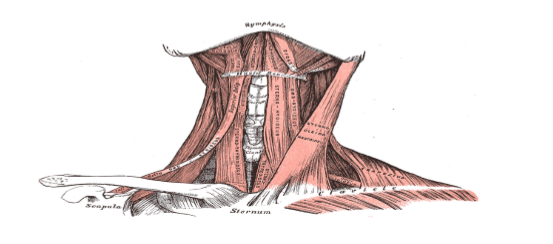
\includegraphics[scale=0.5]{musculosExternosLaringe}
	\caption{Músculos Extrínsecos da Laringe }
	\label{fig:musculoExterno}
\end{figure}

\subsection{Pregas Vocais}

As pregas vocais, como dito anteriormente, estão localizadas dentro da laringe, mais específicamente na parte superior da traqueia. Elas estão posteriormente ligadas às cartilagens aritenoides, e anteriormente ligadas à cartilagem tireoide. As suas bordas exteriores estão ligadas a músculos na laringe, enquanto as suas bordas interiores são livres.

As bordas das pregas vocais são construídas de epitélio, sendo compostas também de algumas fibras musculares. As pregas vocais são bandas triangulares planas de cor branca e acima de ambos os lados destas, se encontram as pregas vestibulares ou falsas pregas vocais. 

O espaço entre as pregas vocais é chamado de glote, sendo que o que está acima da glote é denominado supraglotal e o que está abaixo é denominado subglotal. A Figura 1.5 mostra em mais detalhes a anatomia das pregas vocais, os componentes musculares e as cartilagens atuantes.

\begin{figure}
	\centering
	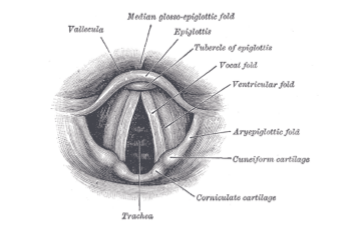
\includegraphics[scale=0.5]{cordasVocais}
	\caption{ Cordas Vocais e Componentes}
	\label{fig:cordasVocasi}
\end{figure}

\section{Fundamentos Biofísicos para a Produção da Voz}
	\subsection{ A Biomecanica da Laringe}
	Primeiramente, devemos ter em mente que o principal papel da laringe não é a produção de voz e sim a proteção das vias respiratórias. Dito isto, podemos fazer uma simples analise, visto que apesar de seu papel principal, a laringe também atua como um instrumento da fala humana. Se analisarmos os instrumentos criados pelo homem podemos notar que estes dependem basicamente de sua geometria, do material que o compõe e da interação de suas partes acústicas. Do mesmo modo, a laringe possui uma determinada geometria, é composta por tecido humano e em conjunto como trato vocal compõe a parte acústica do nosso corpo. Entretanto, nada é tão simples, a sua geometria e as propriedades do material humano envolvidos na produção do som são bastante irregulares\cite{IngoTitze}. 
	
	Outra analogia interessante é sobre o instrumento e quem o utiliza. Um bom pianista por exemplo, sua musica é boa porque ele é habilidoso com o instrumento? Ou sua musica é boa por que o instrumento é bem feito e o som gerado por este é agradável? Ou os dois? Essas perguntas também podem ser feitas com respeito a voz. Para entendermos o que influência na qualidade da síntese da voz é necessário analisar a biomecânica da voz, que nada mais é analisar o movimento do material vivo e as forças atuantes sobre ele\cite{IngoTitze}.
	
	\subsubsection{ Fatores Biológicos que Afetam a Produção de Som na Laringe }
	
	A parte da (bio)mecânica que se relaciona diretamente com a atuação da laringe na produção do som é a mecânica dos meios contínuos, que é a parte da mecânica que lida com a matéria distribuída sobre uma determinada região no espaço, e consequentemente, se contrapõe à mecânica de partículas. Dentro da mecânica de meios contínuos, mais especificamente, a parte que irá nos auxiliar no estudo do comportamento da laringe se chama mecânica de sólidos e fluídos.
	
	Dito isto, analisaremos a seguir alguns conceitos físicos que tem forte ligação com os processos que ocorrem na região da laringe durante a produção do som: 

	\subsubsection{Tensao}
	Tensão é quantidade de força por unidade de área~\cite{IngoTitze} , podemos escrever na forma da equação

	\[
	\sigma = \frac{F}{A}
	\]
	Sendo:
	f : força aplicada. \linebreak
	A: área de aplicação desta força.
	
	\subsubsection{Deformação}
	é a medida de deformação de um meio após a aplicação de uma tensão\citenum{IngoTitze} e pode ser escrito na forma da equação abaixo:
	
	\[
		\epsilon = (L - \frac{L_0}{L_0})
	\]
	
	Onde $\epsilon$ é a medida de deformação, L é o comprimento após a tensão e L0 é o comprimento antes da tensão. Normalmente uma dada deformação em uma dimensão resulta em uma deformação oposta em outra dimensão em um dado meio.
	
	Se uma deformação é uniforme por todo o corpo de um objeto, então chamamos de compressão, se o volume diminui por conta desta deformação, e expansão, se o volume aumenta. 
	
	\subsubsection{Viscosidade}
	É a velocidade de deformação(consequentemente, de restauração) de
	um determinado fluido quando atuam forças de tensão no mesmo. Matematicamente
	pode ser expresso conforme a equação seguinte: \citenum{Ingo}
	
	$
	\sigma = \eta * \frac{d*\epsilon}{dt}
	$
	
	Para $\eta$ viscosidade e t tempo. Quanto maior a viscosidade, mais devagar será a deformação de um meio.
	
	\subsubsection{Elasticidade}
	É uma propriedade do meio que determina quão completa será a restauração do meio após uma dada deformação.
	Os conceitos e propriedades descritos acima são extremamente importantes para se entender a manutenção da produção do som. Como dito anteriormente no capitulo 1, as pregas vocais são músculos e músculos são compostos por fibras, logo, as pregas vocais consistem de uma grande concentração de fibras. Além disso, entre as fíbras que compõe as pregas vocais existem também fluidos atuantes, o que caracteriza as pregas vocais como um material viscoelástico. Para se entender a capacidade de absorção e regeneração das pregas vocais, em detrimento das vibrações de alta frequência e as pressões do ar, deve-se primeiramente estudar as propriedades absorcivas do material que as compõe. Ou seja, em outras palavras, deve-se estudar as propriedades mecânicas do tecido viscoelástico, e
	uma ferramenta que facilita o entendimento é o estudo da curva força-alongamento de um material.
	Entretanto, construir uma curva de força-alongamento depende essencialmente da geometria da amostra do material~\cite{IngoTitze} e, por se tratar de uma material biológico, é difícil obter uma geometria precisa pois as fibras estão constantemente se reorientando em detrimento de lesões e cortes fibrosos. Para viabilizar este estudo, Titze~\cite{IngoTitze} sugere normalizar as forças atuantes e as deformações resultantes para que não haja a dependência direta da geometria. Essa normalização se dá através da substituição da curva força-alongamento por um curva tensão-deformação.
	A Figura\ref{fig:curvaTensaoDeformacao} retirada do estudo feito por Titze~\cite{IngoTitze} demonstra uma curva hipotética de tensão-deformação para os tecidos que compõe as pregas vocais humanas. Esta Figura ilustra o comportamento das fibras das pregas vocais através da relação entre uma força atuante e a deformação gerada por esta. A importância desta analises e deve ao fato de que é possível estabelecer uma relação direta entre nódulos vocais e uma fonação prolongada, alta(em termos de frequência) e intensa.
	A partir da análise desta curva é então possível estabelecer um precedente para a formação de nódulos vocais: a frequência e amplitude da vibração estão diretamente ligadas ao surgimento de um nódulo vocal e consequentemente o de uma fenda pois a força de impacto entre as pregas vocais é proporcional à altura tonal quando acima do tom natural e à intensidade durante a fonação.
	\begin{figure}
		\centering
		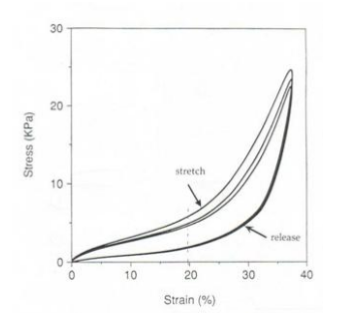
\includegraphics{figura1.png}
		\caption{ Curva Hipotética Tensão-Deformação das Cordas vocais Humanas~\cite{IngoTitze} }
		\label{fig:curvaTensaoDeformacao}
	\end{figure}

	
	\subsection{Reflexão de Som}
	
	Um fenômeno ligado a rigidez e amortecimento entre um meio e outro.\cite{MTAGENTE}
	Ondas quando tentam penetrar em um segundo meio, sendo o segundo meio rígido, as partículas primeiro meio se aglomeram tentando passar porém
	falham, seu acúmulo de particulas geram pressão que acabam criando uma outra onda no primeiro meio decorrente da primeira onda.\cite{HenryGray}
	
	O mesmo ocorre com o meio 2 sendo totalmente não rígido e o primeiro meio sendo bem rígido, Exaurindo excesso de particulas  do meio 1 no meio 2 criando rarefação no meio 1, o que cria uma outra onda de pressão negativa~\cite{FlanaganLandgraf}. A propagação é sempre em direção oposta à fonte, no caso é na direção contrária à coluna de ar(meio 1). 
	
	Para confirmar o precedente supracitado, tomemos a segunda lei de Newton:
	
	\begin{equation}
		\label{eq:1}
		\[ f = \frac{impeto}{periodo}\]
	\end{equation}	
	
	Isto pode ser traduzido em termos de proporção:
	
	\begin{equation}
		\label{eq:2}
		\[ f \propto \frac{impeto}{periodo}\]
	\end{equation}	
	
	Onde m é a massa do tecido das pregas vocais, T é o período de vibração. A velocidade máxima($ V_m $)é proporcional à máxima amplitude e inversamente proporcional ao tempo de fechamento das pregas vocais. Ou seja:
	
	\begin{equation}
		\label{eq:3}
		\[ V_m \propto \frac{A}{T}\]
	\end{equation}	
	
	
	\subsection{Fluxo de Ar na Glote}
	
	Em seções posteriores serão apresentados modelos para representar a vibração das pregas vocais, entretanto para entender por completo esses modelos, devemos antes entender o papel do fluxo de ar nesse processo e para isso devemos analisar primeiro como a pressão de ar é gerada e exercida. À primeira vista, imagine-se que o fluxo de ar é gerado somente pelos pulmões, entretanto, se formos analisar como inspiramos e expiramos percebemos que existem outros fatores contribuintes para a criação e manutenção de um fluxo de ar nas vias respiratórias. O pulmão, como é de se imaginar, é responsável pelo armazenamento do ar e pela troca de oxigênio entre os tecidos que o compõe. Aqui, porém, somente nos interessa esse papel de armazenamento que o pulmão exerce. Ao inspirar o ar, o pulmão aumenta a pressão interna gerando uma tensão aplicada ao tecido elástico que o compõe, a expansão desse tecido gera uma mudança de pressão devido ao aumento do volume pulmonar e à deformação do tecido pulmonar. Em conjunto com essa mudança de pressão, o diafragma, músculo localizado abaixo dos pulmões, é comprimido levando a uma outra mudança de pressão. O diafragma, por sua vez, é um músculo que pode ser controlado, e em virtude disso, é possível controlar a pressão exercida nos pulmões, algo que cantores utilizam para sustentar a técnica vocal. Assim como o diafragma, a caixa torácica também sofre mudanças, expandindo devido ao aumento de volume do pulmão o que gera uma pressão torácica sobre os pulmões. Devido ao fato de ser uma estrutura óssea e portanto ter uma maior rigidez e menor controle se comparado à parede abdominal, a pressão exercida nos pulmões pela caixa torácica é significantemente menor do que a pressão exercida pela aplicação de uma força à parede abdominal. A Figura 2.2 ilustra essa transmissão de pressão por todo o torso citada acima:
	
	\begin{figure}
		\centering
		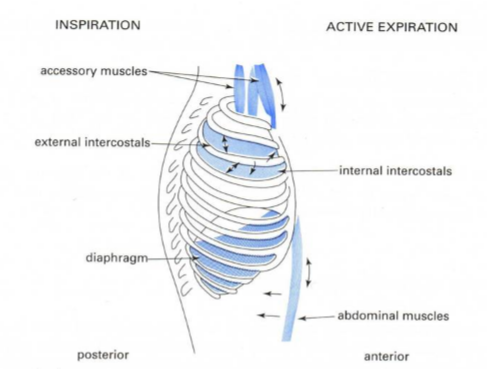
\includegraphics{fluxoDeAr.png}
		\caption{ Pressões Atuantes no Torso~\cite{IngoTitze} }
		\label{fig:fluxoDeAr}
	\end{figure}
		
	Fluxo de ar na Glote:
	
	Como descrito no artigo de Elias temos informações como descobrimos a pressão via fluxo de ar\cite{eliasamadeudesouza}
	
	\[
	U_g = +-(\frac{-a_m}{A_*}+[(a_m)^2 +- (\frac{4K_t}{C^2\rho})](P^+_s - P^-_i))
	\]
	
	\[
	$		A^*  = \text{Área efetiva computada pelas areas A_i e A_s}$
	\]
	
	\[
	$		\rho = \text{Densidade do Ar}$
	\]
	\[
	$		c = \text{Velocidade do som}$
	\]
	
	\[
	$		P_s e P_i = \text{Pressão de incidencia na entra e saída da glote}$
	\]
	
	Uma vez descoberto o fluxo, as pressões de reflexão P^s_ e P^+_i podem ser encontradas com a seguinte equação:
	
	\[
	P^-_s = P^+_s - (\rho c / A_s) U_g
	\]
	
	
	\[
	P^+_i = P^-_i - (\rho c / A_i) U_g
	\]
	
	Quando ocorre o fechamento da glote então alguns parametros assumem valores conhecidos. a(t) = 0 , 
	$P_g = \frac{P_s-P_i}{2}$ e $U_g = 0$	
	
	\subsection{O Sistema Pulmonar}
	
	O sistema pulmonar consiste dos pulmões e vias respiratórias, compostas pela traqueia, glótis e trato vocal. Conforme descrito anteriormente, o tórax e o abdômen em conjunto com o pulmão atuam na geração do fluxo de ar. A glótis, por sua vez, atua como reguladora do fluxo de ar através de variações em seu fechamento que permitem mudanças na pressão envolvida com o movimento do fluxo do ar pelas vias respiratórias. Isso significa que é possível dar constância ao fluxo de ar(Figura 2.3)
	
	
	\begin{figure}
		\centering
		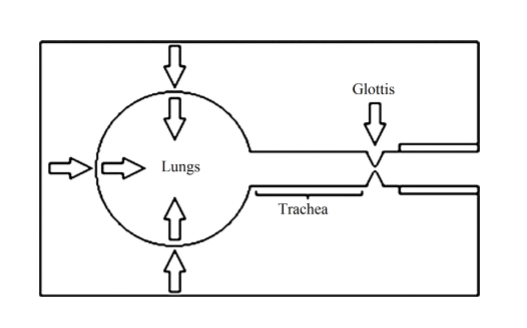
\includegraphics{pulmaoSimplificado.png}
		\caption{ Sistema Pulmonar~\cite{IngoTitze} }
		\label{fig:curvaTensaoDeformacao}
	\end{figure}
		
	\subsubsection{O Processo Físico da Respiração}
	Uma importante lei que nos auxilia no entendimento da relação entre o volume pulmonar e a pressão pulmonar é a Lei de Boyle. A lei nos diz que em um ambiente cujas paredes não são rígidas e em uma temperatura constante, pressão e volume são inversamente proporcionais. Se aplicarmos a lógica dessa lei à respiração humana, fica fácil visualizar o processo físico que envolve a respiração. Quando inspiramos, o diafragma é contraído o que aumenta o volume do pulmão e diminui a pressão interna. Consequentemente, o pulmão se enche de ar. Relacionada à pressão atmosférica, a pressão pulmonar se torna menor, o que gera uma busca pelo equilíbrio das pressões no meio. Esse equilíbrio é alcançado ao se expelir o ar, diminuindo o volume pulmonar e então aumentando a pressão interna novamente. Na verdade é um pouco mais complexo do que isso, entretanto, esse conceito de equilíbrio de pressões é fundamental para o entendimento da abdução e adução das pregas vocais, o que permite a transformação da energia aerodinâmica em energia acústica.
	

	\subsection{Leis de Conservação para Fluxo de Dutos }

	Porém, antes de abordar a transformação de energia aerodinâmica em acústica, é importante se familiarizar com alguns conceitos que regem o comportamento de fluidos em dutos. Isso porque trataremos o fluxo de ar na síntese de voz como um fluído e a modelagem da glote e do trato vocal como a concatenação de pequenos dutos.
	
	\subsubsection{Lei da Continuidade para um Fluxo Incompressível}
	
	
	Quando dizemos que um fluido é incompressível significa dizer que sua densidade não se altera quando este é forçado a passar por uma constrição. Imagine agora um fluido confinado a um duto que possui uma mudança, ao longo de seu comprimento, em sua área transversal formando uma constrição(Figura 2.4). Se não for permitido ao fluido vazar pelas paredes do duto, então todas as partículas do fluido devem ser mantidas mesmo durante a mudança de área transversal ao longo do duto. Para que isso seja possível, as partículas devem acelerar durante a constrição, mantendo-se constante o número de partículas em movimento por unidade de área. Essa relação pode ser expressa pela equação~\ref{eq:4}.
	
	\begin{equation}
		\centering
		\label{eq:4}
		\[
			v_1*A_1 = v_2 * A_2 = constant = U
		\]
	\end{equation}
	
	Onde v e A são respectivamente a velocidade da partícula e a área em que se encontra. U é o fluxo. Matematicamente então, a Lei da Continuidade expressa que um fluxo incompressível em um duto é constante, independente do que acontece com a área transversal ao longo do mesmo~\cite{IngoTitze}
	
	\begin{figure}
		\centering
		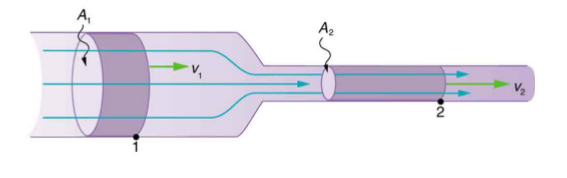
\includegraphics{leiBernoulli.png}
		\caption{ Dinâmica do Fluído em um Duto com Mudança de Área Transversal }
		\label{fig:leiBernoulli}
	\end{figure}
		
	\subsubsection{Lei de Bernoulli área conservação de Energia}
	Outra importante lei de aplicação para o entendimento da síntese de voz é a Lei de Bernoulli para Conservação de Energia. Essa lei foi desenvolvida a partir do reconhecimento de que a energia total atuante no fluido em qualquer ponto durante o trajeto no duto tem duas componentes, a saber, uma energia potencial e uma energia cinética. A energia potencial está relacionada diretamente com a pressão no duto e a energia cinética.
	
	é proporcional ao quadrado da velocidade da partícula. Portanto, podemos expressá-la conforme a equação~\ref{eq:5}.
	
	\begin{equation}
		\centering
		\label{eq:5}
		\[
		P + \frac{1}{2}*\rho* v^2 = constant 
		\]
	\end{equation}
	
	Onde $\rho$ é a densidade do fluido, v a velocidade da partícula e P a pressão no duto. Segue disso o Princípio de Bernoulli: Se a energia em uma corrente de fluido é constante, um aumento na velocidade da partícula deve ser acompanhado de uma queda na pressão~\cite{IngoTitze}.
	
	Analisando a Figura ~\ref*{fig:leiBernoulli}, a pressão na área de constrição deve ser menor que a pressão na área maior do duto, considerando que não hajam perdas de energia no processo. Esse conceito é importante para se compreender o caráter oscilatório das pregas vocais.
	
	\subsubsection{Resistência Glotal}
	
	A resistência a um fluxo é uma característica do sistema de transporte, ou seja, do meio, e pode ser descrita como a razão entre pressão e fluxo(equação\ref{eq:6} )
	
	\begin{equation}
		\centering
		\label{eq:6}
		\[
		R = \frac{P}{U}
		\]
	\end{equation}	
	
	Em sistemas de transporte, as constrições atuam como ponto de resistência a um fluxo. No caso das vias respiratórias humanas, isso normalmente ocorre na glote ou em alguma parte do trato vocal com pouco espaço. Podemos então definir que a resistência glotal será a pressão na glote dividida pelo fluxo que a atravessa. A resistência glotal está diretamente ligada a qualidade vocal pois é responsável por auxiliar no controle do fluxo de ar.

	\section{Oscilação das Pregas Vocais}
	Nesta seção analisaremos os processos e princípios físicos que ocorrem na laringe para que as pregas vocais oscilem, tendo como objetivo destrinchar tais processos a fim de entendermos a reprodução dos mesmos por modelos computacionais utilizados para simulação da voz humana. Os primeiros estudos sobre vibração das pregas vocais especulavam que as pregas vocais se ajuntavam por um efeito de pressão negativa(Princípio de Bernoulli) na glote. A esta descrição de vibração nas pregas vocais se deu o nome de Teoria Mioelástica Aerodinâmica da Vibração das Pregas Vocais, conhecida também pelo nome de seu criador como Teoria de van der Berg . A teoria de van der Berg serviu como marco para o desenvolvimento teórico do campo de estudos da voz e consequentemente o aparecimento dos primeiros modelos matemáticos de representação do funcionamento das pregas vocais. Entretanto, apesar disso, sua teoria é inadequada para explicar a vibração auto sustentável das pregas vocais~\cite{FlanaganZueiro}. Isso porque as forças de Bernoulli por si só não são capazes de distinguir entre os movimentos interiores e posteriores das pregas vocais. Assim sendo, são necessários mecanismos para prover um aumento ou decréscimo às forças de Bernoulli durante a abertura e o fechamento das pregas vocais respectivamente, caso contrário, as oscilações serão amortecidas.
	
	
	
	

	\subsection{Lei Bernouli}
		Energia potencial e energica cinética em fluídos se mantém a mesma
		porém em proporções diferentes \cite{BradhStory}:
		
		\[
		P + \frac{\rho * v^2}{2} = Constante\\
		Sendo: \\
		\rho = Densidade do fluido \\
		P = Pressão no duto onde o fluído se encontra\\
		v =  velocidade da particula 
		\]
	\subsection{Critérios para Oscilação}
		Alguns critérios devem ser atendidos para que um determinador padrão de movimento seja considerado como uma oscilação mecânica, a saber:
		
		
		No sistema onde ocorre o movimento deve haver uma posição de equilíbrio estável, que é caracterizada por uma força restaurativa que sempre acelera o corpo em	movimento de volta para a sua posição de repouso.
		Deve haver inércia(no caso do sistema mecânico, a massa atua como propriedade de inércia) no sistema para superar esta posição de equilíbrio.
		A perda, em excesso, de energia por ciclo de oscilação deve ser zero.\ldots 
	
	\subsection{Tipos de Oscilação}
			De acordo com Titze~\cite{IngoTitze}, os tipos de oscilação são:
			\begin{itemize}
				\item  Oscilação Natural: Quando um sistema que se encaixa nos critérios anteriores se move sem interferência após um distúrbio inicial.
				\item Oscilação Natural: Quando um sistema que se encaixa nos critérios anteriores se move sem interferência após um distúrbio inicial.
				\item Oscilação Forçada: Requer uma fonte externa de condução que por si só é um
				oscilador. Dita grande parte do padrão de vibração do sistema.
				\item Oscilação Auto-Sustentável: Requer uma fonte de energia estável e uma interação não-linear entre os componentes internos ao sistema. As perdas de energia são compensadas, mantendo o padrão oscilatório.
			\end{itemize}
		






	\section{Sistema Auditivo}
	\subsection{Introdução}
	O Sistema auditivo consiste em componentes periféricos e centrais.Atualmente a maior parte do conhecimento do funcionamento dos sistemas auditivos deriva de estudos de animais não humanos.\cite{Foundation1} 
	
	Sistema auditivo diferencia-se entre espécies em jeitos interessantes.
	Por exemplo algumas espécies tem caracteristicas diferentes relacionadas aos sinais vocais mais utilizados por ela mesma.\cite{Foundation1}
	
	\subsection{Intensidade}
	Como a frequência de um estímulo a intensidade dele é processado e codificado sub-cortical nos dois lados do cérebro em todos os níveis no cerébro.\cite{Foundation1}
	
	
	
	\section{Voz e Propriedades Linguísticas}
	Uma divisão importante de acordo com Flanagen, são as letras separados em classificações Vogais e Consoantes que se associam a um movimento do trato vocal correspondente~\cite{JFlanagan}.
	
	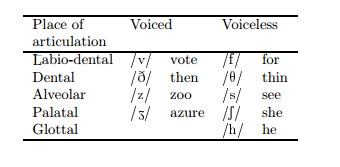
\includegraphics{tabelaConsoantes.png}
	
	\subsection{Vogais}
	
	O trato vocal ao produzir uma vocal, em um articação normal, mantém-se relativamente estável.Há uma opção de contribuição das cavidades nasais, uma cobertura porém é negligenciável.Baseado nessas caracteristicas é divididos todas as consonantes. A tabela abaixo explica:
	
	
	\subsection{Consoantes}
	Sons produzidos com constrições em algum ponto no trato vocal. Dividido em quatro (4) classes, baseados em duas funcionalidades binárias, sonorant e continuant.
	
	
	\subsubsection{Sonorant}	 
	Sonorant pode ser traduzido como "cantado". Consoantes Sonorant são sons que não aumentam a pressão do ar dentro do trato vocal pois a constrição não é muito justa ou o palato continua aberto, deixando ar escapar por ele.
	
	\subsubsection{Continuant}
	Uma consoante discontinuant é produzida por um fechamento completo em algum ponto no trato vocal.
	

 

